\documentclass[11pt]{article}

\usepackage[utf8]{inputenc}
\usepackage[spanish]{babel}
\usepackage{a4wide}
\usepackage{graphicx}

\title{Trabajo obligatorio Métodos Numéricos I Resonancia en oscilaciones no lineales}
\author{Unai Aguilera Irazabal\\ DNI: 45663055M}

\begin{document}
\maketitle

\section{Introducción}
La ecuación diferencial (\ref{ecuacion-diferencial}), proporcionada en el enunciado del trabajo, modela un oscilador no lineal en su forma más general.

\begin{equation}
\label{ecuacion-diferencial}
	 \frac{d^2 x}{dt^2} + \gamma\frac{dx}{dt} + \omega_{o}^2x + \beta{}x^2 = F_{o}\cos{\omega{}t}
\end{equation}

El primer término del primer miembro de la ecuación representa la aceleración que sufre el oscilador durante su movimiento. El segundo término
define el amortiguamento del oscilador debido a la aplicación de fuerzas que no son conservativas, como puede ser el caso del rozamiento. Dicho término es proporcional a la velocidad del oscilador en cada instante y está regulado por el coeficiente $\gamma$.

El tercer miembro es la fuerza lineal que es aplicada sobre el oscilador y que tiene naturaleza armónica. Este termino es proporcional a la frecuencia natural del oscilador $\omega_{o}$ que viene determinada por las características físicas del mismo: masa, longitud del péndulo, constante elástica del muelle, longitud del péndulo, etc.

El último termino del primer miembro introduce las características no lineales del oscilador mediante la aplicación de fuerzas que dependen del cuadrado de la posición del oscilador en cada instante.

Por último, el segundo miembro de la ecuación representa la aplicación de una fuerza externa sobre el oscilador de naturaleza periódica y con una frecuencia $\omega$.

\section{Resolución numérica}

\subsection{Método de Runge-Kutta}
Para la resolución de la ecuación diferencial no lineal planteada en el trabajo se ha optado por la aplicación de un método númerico para la integración de ecuaciones diferenciales. Este tipo de métodos permite obtener una solución numérica en aquellos casos en los que no es posible llevar a cabo la resolución de la ecuación diferencial por métodos analíticos. De una forma general, la obtención de la solución númerica de una ecuación diferencial se basa en la aproximación del siguiente valor de la función mediante incrementos muy pequeños de la variable independiente y utilizando para ello la información proporcionada por la derivada primera de la función. La derivada de la función es evaluada en cada paso, obteniéndose la nueva razón del incremento de la variable dependiente para el siguiente. Se obtiene así una tabla que contiene los valores de la función en determinados valores de la variable independiente, normalmente esquipaciados entre sí debido a la utilización de un paso constando.

Como el enunciado del trabajo requiere un método numérico de cuarto orden, se ha aplicado el método Runge-Kutta de dicho orden de acuerdo a su definición en la página 460 del libro de Gerald \& Wheatley \textit{Análisis numérico con aplicaciones}. En el método de Runge-Kutta, aplicado a la resolución de una ecuación diferencial del tipo $\frac{dy}{dx}$, el incremento en $y$ no es proporcional unicamente al valor de la derivada en el punto anterior, sino a un promedio ponderado de varias estimaciones de dicho incremento. En el caso concreto del método de cuarto orden se obtiene un promedio ponderado de cuatro estimaciones $k_n$ calculada cada una de ellas utilizando la información de las $k_{n -1}$. 

El método de Runge-Kutta de cuarto orden para la resolución de una ecuación diferencial de primer grado queda definido por el siguiente conjunto de ecuaciones:

\begin{equation}
	k_1 = hf(x_n, y_n)
\end{equation}

\begin{equation}
	k_2 = hf(x_n + \frac{1}{2}h, y_n + \frac{1}{2}k_1)
\end{equation}

\begin{equation}
	k_3 = hf(x_n + \frac{1}{2}h, y_n + \frac{1}{2}k_2)
\end{equation}

\begin{equation}
	k_4 = hf(x_n + h, y_n + k_3)
\end{equation} 

\begin{equation}
	y_{n+1} = y_{n} + \frac{1}{6}(k_1 + 2k_2 + 2k_3 + k_4)
\end{equation}

\subsubsection{Método de Runge-Kutta para ecuaciones diferenciales de segundo grado}
Para poder aplicar el método anterior a la resolución numérica de ecuaciones diferenciales de segundo grado, como es el caso del oscilador anarmónico, es necesario, primeramente, llevar a cabo una descomposición de la ecuación planteada en un sistema de dos ecuaciones diferenciales
de primer grado, de acuerdo a lo explicado en las páginas 477-478 del libro de Gerald \& Wheatley. 

En el caso de la ecuación (\ref{ecuacion-diferencial}) del problema propuesto, la realización de la substitución $\frac{dx}{dt} = y$, permite obtener el siguiente sistema de ecuaciones:

\begin{equation}
	\frac{dx}{dt} = y = f(t, x, y)
\end{equation}

\begin{equation}
	\frac{dy}{dt} = F_{o}\cos{\omega{}t} -\gamma{}y - \omega_{o}^2x - \beta{}x^2 = g(t, x, y) 	
\end{equation}

donde se han indicado también las funciones $f(t, x, y)$ y $g(t, x, y)$ se utilizarán para la aproximación.  

Por otro lado, el método de Runge-Kutta explicado anteriormente debe ser modificado para poder ser aplicado al sistema de ecuaciones diferenciales de forma correcta, tal y como se explica en la página 480 del libro de Gerald \& Wheatley. En este caso se alterna en la obtención de las constantes $k_n$ para cada una de las ecuaciones, y se utilizan los valores correspondientes a cada variable dependiente
para el incremento durante el cálculo de la siguiente constante. Así, las ecuaciones de Runge-Kutta para el caso de un sistema de dos ecuaciones son de la siguiente forma:

\begin{equation}
	k_1 = hf(t_n, x_n, y_n)
\end{equation}

\begin{equation}
	l_1 = hg(t_n, x_n, y_n)
\end{equation}

\begin{equation}
	k_2 = hf(t_n + \frac{1}{2}h, x_n + \frac{1}{2}k_1, y_n + \frac{1}{2}l_1)
\end{equation}

\begin{equation}
	l_2 = gf(t_n + \frac{1}{2}h, x_n + \frac{1}{2}k_1, y_n + \frac{1}{2}l_1)
\end{equation}

\begin{equation}
	k_3 = hf(t_n + \frac{1}{2}h, x_n + \frac{1}{2}k_2, y_n + \frac{1}{2}l_2)
\end{equation}

\begin{equation}
	k_3 = gf(t_n + \frac{1}{2}h, x_n + \frac{1}{2}k_2, y_n + \frac{1}{2}l_2)
\end{equation}

\begin{equation}
	k_4 = hf(t_n + h, x_n + k_3, y_n + l_3)
\end{equation}

\begin{equation}
	k_4 = hf(x_n + h, x_n + k_3, y_n + l_3)
\end{equation} 

\begin{equation}
	x_{n+1} = x_n + \frac{1}{6}(k_1 + 2k_2 + 2k_3 + k_4)
\end{equation}

\begin{equation}
	y_{n+1} = y_n + \frac{1}{6}(l_1 + 2l_2 + 2l_3 + l_4)
\end{equation}

\subsubsection{Estudio de la precisión del método de Runge-Kutta}
\label{precision-runge-kutta}

\subsection{Transformada de Fourier}

\section{Casos de estudio}
Se exponen a continuación los resultados del estudio realizado tanto de la forma de la señal como del espectro de potencias para cada uno de los siguientes casos de la ecuación \ref{ecuacion-diferencial}:

\begin{itemize}
	\item Oscilador lineal no forzado ni amortiguado ($\gamma = \beta = F_o = 0$).
	\item Oscilador lineal forzado pero no amortiguado ($\gamma = \beta = 0$ pero $F_o \neq 0$).
	\item Oscilador lineal forzado y amortiguado ($\beta = 0$ pero $\gamma \neq 0, F_o \neq0$).
	\item Oscilador no lineal forzado y amortiguado ($\gamma \neq 0, \beta \neq 0, F_o \neq 0$).
\end{itemize}

Aunque los tres primeros casos pueden ser resueltos de forma analítica para encontrar la solución exacta, se ha llevado a cabo la resolución numérica de los diferentes casos para comprobar que los métodos implementados se comportan de la forma esperada en cada caso. Para el estudio de todos los casos anteriores se han considerado las siguientes condiciones iniciales:  $x(0) = \frac{dx}{dt}(0) = 0$.

\subsection{Oscilador lineal no forzado ni amortiguado}
En la sección \ref{precision-runge-kutta} se ha llevado a cabo un estudio de la precisión del método de integración numérica para la resolución del sistema de ecuaciones. En el caso de que se apliquen las condiciones iniciales consideradas, debido a que el oscilador armónico se encuentra inicialmente en reposo y sobre el no actua ninguna fuerza, no se producirá ningun cambio en su situación a lo largo del tiempo. Debido a que no existe ningún movimiento armónico del oscilador las frecuencias constitutivas del mismo tienen todas valor exactamente cero. Ambos resultados se observan en la figura \ref{fig:caso_lineal}.

\begin{figure}
\label{fig:caso_lineal}
\centering
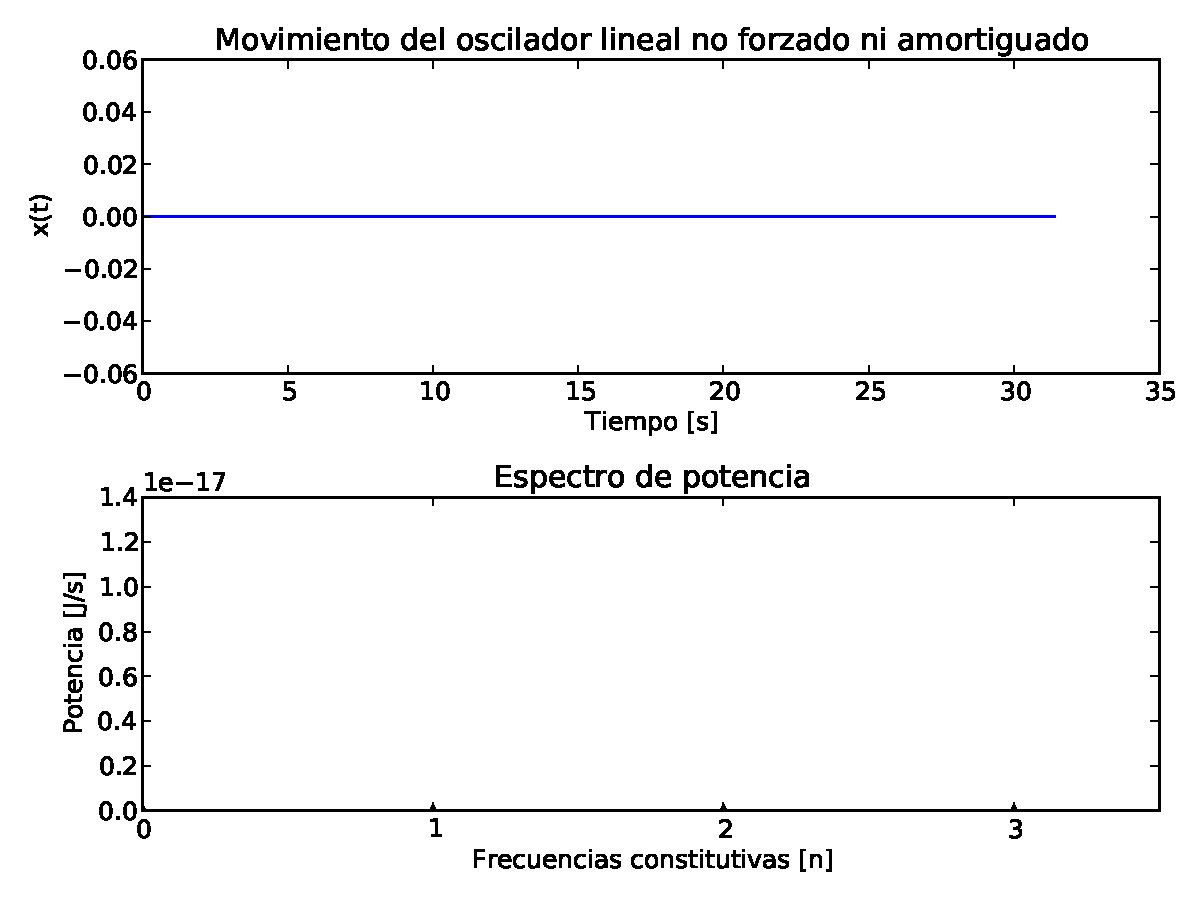
\includegraphics[width=0.75\linewidth]{caso_lineal.pdf}
\caption{Representación de la señal y espectro de potencias para un oscilador lineal no forzado ni amortiguado. La señal ha sido obtenida mediante la aplicación del método de Runge-Kutta de cuarto orden y con un paso de integración $h = 0.01$}
\end{figure}

\end{document}